% +--------------------------------------------------------------------+
% | Sample Chapter 2
% +--------------------------------------------------------------------+

\cleardoublepage

% +--------------------------------------------------------------------+
% | Replace "This is Chapter 2" below with the title of your chapter.
% | LaTeX will automatically number the chapters.
% +--------------------------------------------------------------------+

\chapter{Estado del arte}
\label{makereference2}
En esta sección de la memoria procederemos a describir las tecnologías que hemos implementado
en nuestro trabajo, tales como la \textbf{realidad aumentada}, las distintas \textbf{fuentes de información}, 
\textbf{técnicas de recomendación}, junto a una serie de análisis de las \textbf{necesidades de los usuarios} y de la \textbf{competencia}.
\section{Realidad Aumentada}
\label{makereference2.1}
Según el enlace de Wikipedia: \url{https://es.wikipedia.org/wiki/Realidad_aumentada}, la \textbf{realidad aumentada} es el término que se 
usa para describir al conjunto de tecnologías que permiten que un usuario visualice parte de mundo real a través de un dispositivo tecnológico 
con información gráfica añadida por éste dispositivo. Este dispositivo o conjunto de dispositivos, añaden información virtual a la información 
física ya existente; es decir, una parte sintética virtual a la real. Podemos estar de acuerdo en que es una tecnología en auge actualmente, sobre todo 
en el uso de los \textbf{smartphones} ya que prácticamente todas las personas poseen uno. Esta tecnología nos permite añadir un valor importante a 
nuestra aplicación, por lo que consideramos que el grueso de nuestro proyecto se centra en ella. Los casos de uso más importantes de nuestra aplicación 
usarán la \textbf{realidad aumentada} para proveer al usuario de información adicional y de gran relevancia de las imágenes que reconozca, ya sean carteles
de películas o caras de usuarios que usen la aplicación.
\subsection{Tecnologías actuales}
\label{makereference2.1.1}
\paragraph{ARCore:}
Plataforma creada por Google para desarrollar aplicaciones de
 realidad aumentada con soporte para Android, Android NDK, iOS,
 Unity y Unreal Engine. Aunque las funcionalidades que se ofrecen
 para iOS y Unity for iOS se limitan a Cloud Anchors, los anchors
 sirven para hacer que objetos virtuales aparezcan en un lugar
 captado por la cámara de nuestro dispositivo estos son compartidos
 en la nube para que multitud de dispositivos disfruten de la misma
 experiencia, los dispositivos con iOS podrán usarlos utilizando ARKit.

Tiene una curva de aprendizaje media y con su versión 1.5 demuestra una
 estabilidad interesante respecto a su reciente creación. Cabe destacar
 que no todos los dispositivos son compatibles, esto depende de que las
 empresas que desarrollan estos dispositivos cumplan unos requisitos
 para asegurar que la experiencia con ARCore es la adecuada y de la
 versión del sistema operativo. se puede ver con más detalle en esta
 dirección \url{https://developers.google.com/ar/discover/supported-devices}.

ARCore usa tres características a través de la cámara del dispositivo:
 \begin{itemize}  
     \item {\bf Motion tracking} permite al dispositivo entender y rastrear la posición relativa del mundo.
     \item {\bf Environmental understanding} permite al dispositivo detectar el tamaño y localización de todos los tipos de superficies.
     \item {\bf Light estimation} permite al dispositivo estimar las condiciones de luz del entorno actual.
 \end{itemize}

\paragraph{ARKit:}
Podemos utilizar experiencias de realidad aumentada persistente, compartirlas entre distintos dispositivos iOS,
 detecta imágenes 2D incluso en movimiento y objetos 3D.

\paragraph{Wikitude:}
Kit de desarrollo para realidad aumentada con soporte para Android, iOS, Unity, Cordova, Xamarin (mala
 documentación y versiones obsoletas), Titanium, React Native.
Su licencia es de pago, aunque hay versiones limitadas gratuitas.
Utiliza ARCore o ARKit cuando los dispositivos lo soportan y en caso de que no utiliza tecnología de Wikitude
 para que el número de dispositivos compatibles sea mayor. 

\paragraph{Vuforia:}
Kit de desarrollo para realidad aumentada con soporte para Android, iOS, UWP y Unity.
Software de pago solo permite usarse gratis para pruebas.

\paragraph{ViroReact:}
Plataforma para construir aplicaciones con realidad aumentada usando React Native.
 Utiliza ARKit y ARCore para dotar a las aplicaciones de una experiencia de RA sin
 utilizar código distinto y con una curva de aprendizaje fácil. Al basarse en React
 Native que no tiene versión estable provoca problemas con las versiones de dependencias,
 configuraciones tediosas y largas compilaciones.
Es un software privativo gratuito.

\paragraph{Expo AR:}
API que permite crear aplicaciones en React Native utilizando ARKit únicamente.
Está en una fase muy inicial.

\section{Análisis de la competencia}
\label{makereference2.2}
\begin{flushleft}
    Consideramos que la aplicación que hemos diseñado consta de dos partes claramente diferenciadas (la parte de \textbf{Realidad Aumentada} 
    y la parte de \textbf{Recomendación y gestión} de películas), consideramos que existen distintos tipos de competencia dependiendo de cada una de ellas.
     \begin{itemize}  
         \item En la parte de recomendación y gestión de películas, compite claramente con aplicaciones como \textbf{IMDB} o \textbf{MovieBase}. 
         Estas aplicaciones proporcionan, herramientas para guardar películas y recomendar éstas a los usuarios en función de sus gustos. Estas funcionalidades son 
         muy parecidas a las que nosotros hemos decidido proporcionar a nuestros usuarios, con la diferencia que nuestra aplicación, además de las funcionalidades anteriormente 
         mencionadas, permite realizar más acciones sobre las películas como crear planes con amigos.
        \item A diferencia de la parte de recomendación y gestión en donde hay una gran variedad de aplicaciones que ofrecen servicios parecidos a los nuestros, únicamente hemos 
        encontrado una aplicación (\textbf{Paramount AR+}) que ofrezca servicios parecidos a los nuestros relacionados con Realidad Aumentada. Según las especificaciones de la aplicación permite identificar pósteres y 
        mostrar información sobre la película detectada, servicio muy parecido al que nosotros hemos proporcionado. 
    \end{itemize}
    Para intentar alejarnos de esta competencia, hemos decidido unir ambas funcionalidades en una aplicación y, además, proporcionar al usuario más funcionalidades como escanear una aplicación con Realidad Aumentada, 
    ver su información y añadirla a un plan con amigos para ver dicha película. Para funcionalidades como ésta y otras en las que unimos la realidad aumentada con la recomendación de películas y gestión de planes no hemos encontrado actualmente ninguna aplicación que proporcione estos servicios.
    \\
    Además, una funcionalidad nuestra aplicación proporciona y no hemos encontrado otra que lo haga es la gestión de amigos con Realidad Aumentada. 
    Como que al enfocar con la cámara a un amigo y que en la misma pantalla de realidad Aumentada muestre visualmente la información de los tres planes activos que tiene mi amigo que más podrían gustarme y cuanto se estima que me gustaría ese plan.
    \begin{figure}[H]
        \centering
        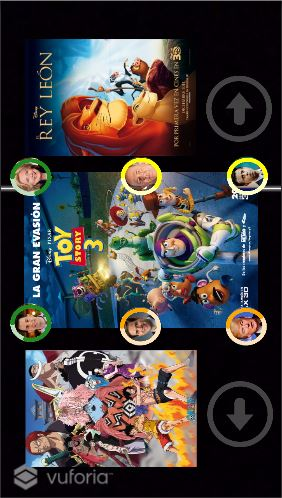
\includegraphics[width=3in, angle=270]{figures/chapter-2/recomendadorAR.JPG}
        \caption{Vista encargada de recomendar planes en RA al enfocar a un amigo}
    \end{figure}
    
\end{flushleft}
\newpage
\section{Fuentes de información}
\label{makereference2.3}
Como nuestra aplicación muestra información sobre las películas que se recomiendan y que los usuarios han guardado, hemos
tenido que investigar de que página web podríamos obtener estos datos tan relevantes.
\paragraph{IMDB:}
Nos decidimos por usar la página web de \textbf{IMDB}: \url{https://www.imdb.com/} para conseguir las valoraciones, resúmenes, nombre del director,
género y país de las películas, entre otros datos, debido a que consideramos que es de las webs más usadas entre los cinéfilos y posibles 
usuarios de nuestra aplicación.

\section{Técnicas de recomendación}
\label{makereference2.6}



